% =====================================================================
%  Prabhavit Gupta - Tailored CV for Data Engineer at Capgemini
%  Target: Capgemini (Modern Data Platforms, Data Pipelines, AI Ecosystems)
%  Compile: tectonic cv/main_Capgemini_DataEngineer.tex
%  Rules: ONE PAGE. No unicode em-dashes. Verified facts. ATS-optimized.
% =====================================================================
\documentclass[a4paper,10pt]{article}

\usepackage[T1]{fontenc}
\usepackage[utf8]{inputenc}
\usepackage[top=0.8cm,bottom=0.8cm,left=1.0cm,right=1.0cm]{geometry}
\usepackage{titlesec}
\usepackage{enumitem}
\usepackage{hyperref}
\usepackage{xcolor}
\usepackage{graphicx}

\definecolor{accent}{HTML}{1F4E78}
\hypersetup{colorlinks=true, urlcolor=accent, linkcolor=accent}
\pagestyle{empty}
\setlength{\parindent}{0pt}

\titleformat{\section}{\large\bfseries\color{accent}}{}{0em}{}[\vspace{-0.6em}\rule{\textwidth}{0.8pt}]
\titlespacing{\section}{0pt}{2pt}{1pt}

\newcommand{\role}[4]{%
 \textbf{#1} \hfill \textbf{#2}\\[1pt]%
 \textit{#3} \hfill \textit{#4}\\[2pt]%
}
\setlist[itemize]{leftmargin=1.2em, itemsep=0pt, topsep=1pt, parsep=0pt}

\begin{document}

% ================= HEADER =================
\begin{minipage}[c]{0.80\textwidth}
 {\Huge\bfseries Prabhavit Gupta}\\[3pt]
 {\color{accent}\large Data Engineer: Modern Data Platforms, Ingestion Pipelines \& AI Systems}\\[6pt]
 {\footnotesize +39 351 610 7807 ~$\vert$~
 \href{mailto:prabhavitg@gmail.com}{prabhavitg@gmail.com} ~$\vert$~
 \href{https://www.linkedin.com/in/prabhavit/}{linkedin.com/in/prabhavit} ~$\vert$~
 \href{https://github.com/prab-gupta}{github.com/prab-gupta} ~$\vert$~
 Venice, Italy}
\end{minipage}\hfill
\begin{minipage}[c]{0.18\textwidth}
 \raggedleft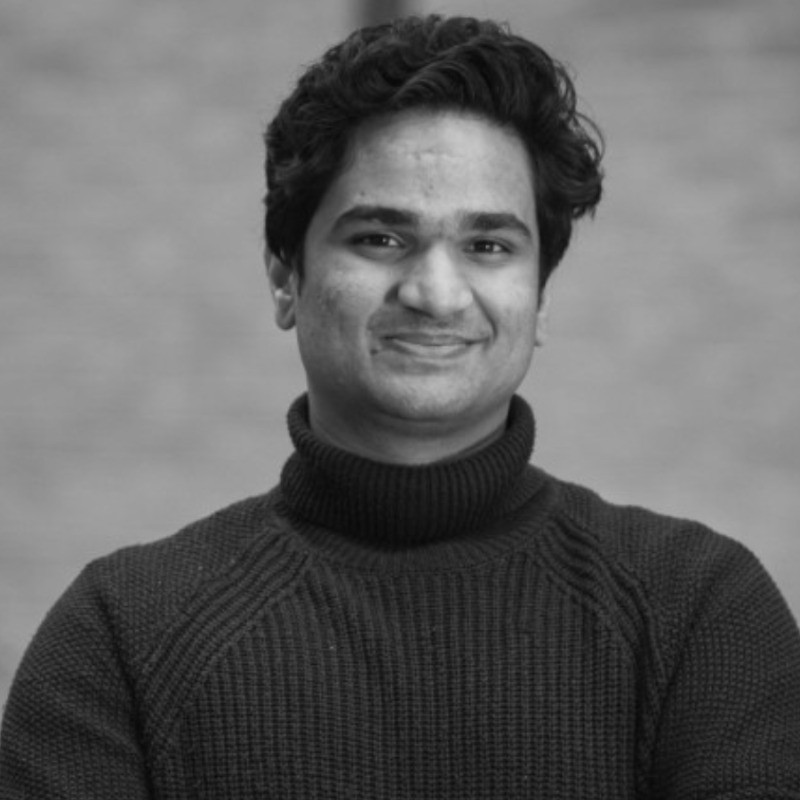
\includegraphics[width=2.0cm]{photo.jpg}
\end{minipage}
\vspace{-2pt}

% ================= SUMMARY =================
\section{Summary}
Data Engineer who builds automated data pipelines, relational data architectures, and ingestion workflows that transform multi-format, unstructured inputs into production data assets. At FlowSpace, led the core platform and data migration from a legacy architecture to modern PostgreSQL and Laravel schemas, engineered an automated ingestion pipeline processing 900+ entities with data quality validation, and deployed live query agents on transactional databases. Daily tools are Python, SQL, TypeScript, Docker, and REST APIs.

% ================= SKILLS =================
\section{Skills}
\begin{itemize}
 \item \textbf{Data Pipelines \& Integration:} ETL/ELT pipelines, multi-format data ingestion (PDF, spreadsheet, web to structured JSON/relational schemas), data quality and validation, event-driven workflows, n8n, automated error recovery, REST APIs, webhooks
 \item \textbf{Data Architecture \& Storage:} PostgreSQL, MySQL, Supabase, NoSQL, relational data modeling, schema migration, Modern Data Platform principles, DWH concepts, familiarity with Lambda/Kappa and Data Mesh architectures
 \item \textbf{Languages, Tools \& AI Systems:} Python, SQL, TypeScript, JavaScript, Docker, Git, CI/CD; familiar with Apache Spark and Kafka; RAG vector pipelines, LLM-driven structured extraction (Claude, OpenAI), AI agents querying live operational databases
\end{itemize}

% ================= EXPERIENCE =================
\section{Experience}

\role{\href{https://flowspace.co}{FlowSpace.co}}{Mar 2024 -- Aug 2026}{Lead Data \& Full-Stack Engineer (Full-time, Freelance)}{London, UK (remote)}
\begin{itemize}
 \item Led the core data migration off a legacy architecture to a modern PostgreSQL, Next.js and Laravel stack, executing entity-level mapping and automated cutover scripts while scaling from 2,000 to 4,500+ active users.
 \item Architected an automated data ingestion pipeline (TypeScript, n8n, Claude API) extracting, normalizing, and validating multi-format inputs (PDFs, spreadsheets, web feeds) into structured schemas (900+ listings processed).
 \item Engineered bidirectional REST API integrations and webhook pipelines with OfficeRnD and Nexudus for automated booking synchronization and data consistency.
 \item Deployed AI support agents querying live transactional records with confidence scoring and automated human escalation.
\end{itemize}

\role{\href{https://get2germany.com}{Get2Germany.com}}{Jan 2024 -- May 2024}{Developer \& Automation Specialist (Part-time)}{Berlin, Germany}
Engineered automated data collection workflows in n8n, integrated Google APIs, and optimized database queries and schema performance.\\[1pt]

\role{\href{https://clubee.com}{Clubee.com}}{Sep 2023 -- Aug 2024}{Developer \& QA (Full-time, Freelance)}{Foetz, Luxembourg}
Integrated Clubee REST APIs across platforms, developed data validation suites and federation dashboard tools, and conducted QA verification.\\[1pt]

\role{\href{https://tractionboard.co}{Tractionboard.co}}{Aug 2023 -- Oct 2023}{Developer (Internship)}{Utrecht, Netherlands}
Integrated OpenAI and SendGrid APIs for automated data processing, implemented responsive data views, and resolved production bugs.

% ================= FREELANCE PROJECTS =================
\section{Selected Projects}
\begin{itemize}
 \item \textbf{\href{https://smarturlink.com/}{Urlink}} (2025), Project Manager \& Developer. Modeled PostgreSQL schemas on Supabase, designed platform business logic, and automated client data synchronization workflows. Stack: Next.js, Supabase, Netlify.
 \item \textbf{\href{https://ultrastrategy.com}{UltraStrategy}} (2024 to 2025), AI Automation Developer. Built an automated document-parsing ETL pipeline using n8n and Eden AI for multi-source data extraction into structured candidate profiles.
 \item \textbf{\href{https://github.com/prab-gupta/llm-doc-parser}{LLM Document Parser}} (Open Source), Creator. Engineered a public pipeline parsing semi-structured and unstructured documents into strictly validated JSON schemas.
\end{itemize}

% ================= CERTIFICATIONS =================
\section{Certifications}
Microsoft Copilot Studio Agent Academy \textbullet\ Microsoft: Introduction to building AI agents \textbullet\ Microsoft Power Automate \textbullet\ Tray.AI Build Practitioner (Sep 2024)

% ================= EDUCATION =================
\section{Education}
\textbf{Ca' Foscari University of Venice} \hfill Oct 2020 -- Jun 2024\\
BA Philosophy, International Studies \& Economics (Minor: Entrepreneurship)

% ================= AUTH =================
\vspace{2pt}
{\small \textbf{Work authorization:} European Long Term Residence Permit (Italy); available immediately. \quad \textbf{Languages:} Hindi (native), English (fluent / C2), Italian (conversational).}

\end{document}
